
\part{Un processeur fictif}

\section{Exemple pédagogique}
\begin{frame}
\frametitle{Un processeur fictif}  

\structure{Éléments}
\begin{itemize}
\item machine à mots de 16 bits, adresses sur 12 bits
\item 1 accumulateur 16 bits
\item compteur ordinal 12 bits 
\item jeu de 13 instructions sur 16 bits 
  \begin{itemize}
    \item arithmétiques : addition et soustraction 16 bits, complément à 2.
    \item chargement et rangement directs et indirects
      \item saut conditionnel et inconditionnel, appel de sous-programme
      \item ...
  \end{itemize}
\end{itemize}
\end{frame}


\section{Jeu d'instructions}

\begin{frame}
  \frametitle{Format des instructions}

  1 instruction = 16 bits. Format unique : 
\begin{itemize} 
\item \alert{code opération} sur 4 bits (poids forts)
\item \alert{opérande} sur 12 bits
\end{itemize}

\begin{center}
\begin{tabular}{|c|c|}
\hline
code & opérande \\
4 bits & 12 bits \\
\hline
- - - - & - - - - - - - - - - - - \\
\hline
\end{tabular}
\end{center}
\end{frame}

\begin{frame}
  \frametitle{exemple}
Le mot \fbox{\texttt{0011 0000 0110 0100}} (\texttt{Ox3064})
peut représenter une \alert{instruction} 
\begin{itemize}
\item  de code \fbox{\texttt{0011}} = 0x3 
\item d'opérande \fbox{\texttt{0000 0110 0100}} = 0x064 (100 en décimal)
\end{itemize}
\begin{multicols}{2}
qui signifie  ``\emph{ranger le contenu de l'accumulateur dans le mot mémoire d'adresse 100''}
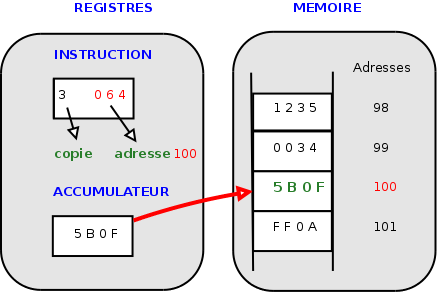
\includegraphics[width=1\linewidth]{figures/store-100.png}
\end{multicols}
\end{frame}

\begin{frame}
  \frametitle{Instruction ou donnée ?}

Le mot 0x3064 représente :
\begin{itemize}
\item une \alert{instruction} (code 3, opérande 100)
\item le \alert{nombre +12388} en binaire complément à 2 
\end{itemize}

La signification d'un mot en mémoire dépend de ce qu'on en fait.
\end{frame}


\begin{frame}[containsverbatim]
  \frametitle{Le jeu d'instructions}


\begin{center}
\footnotesize
\begin{tabular}{|lllll|}
\hline
 & Mnémonique &  Description & Action & \texttt{Cp = } \\
\hline
0 & \texttt{loadi} \emph{imm12} &  \alert{chargement} immédiat &  \verb/Acc = ext(imm12)/ & \verb/Cp + 1/\\
1 & \texttt{load} \emph{adr12} &  chargement direct &  \verb/Acc = M[adr12]/ & \verb/Cp + 1/ \\
2 & \texttt{loadx} \emph{adr12} &  chargement indirect &  \verb/Acc = M[M[adr12]]/& \verb/Cp + 1/ \\
\hline
3 & \texttt{store} \emph{adr12} &  \alert{rangement} direct &  \verb/M[adr12] = Acc/ & \verb/Cp + 1/ \\
4 & \texttt{storex} \emph{adr12} &  rangement indirect &  \verb/M[M[adr12]] = Acc/& \verb/Cp + 1/ \\
\hline
5 & \texttt{add} \emph{adr12} & \alert{addition} & \verb/Acc += M[adr12]/ & \verb/Cp + 1/ \\
6 & \texttt{sub} \emph{adr12} & \alert{soustraction} & \verb/Acc -= M[adr12]/ & \verb/Cp + 1/ \\
\hline
7 & \texttt{jmp} \emph{adr12}  & \alert{saut} inconditionnel & &\verb/adr12/  \\
8 & \texttt{jneg} \emph{adr12}  & saut si négatif & & si \verb/Acc < 0/ \\
  & & & & alors \texttt{adr12} \\
  & & & & sinon \texttt{Cp+1}  \\
9 & \texttt{jzero} \emph{adr12}  & saut si zero & & si \verb/Acc==0/ \\
  & & & & alors \texttt{adr12} \\
  & & & & sinon \texttt{Cp+1}  \\
\hline
A & \texttt{jmpx} \emph{adr12}  & saut indirect & & \verb/M[adr12]/ \\
B & \texttt{call} \emph{adr12}  & \alert{appel} & \verb/M[adr12] = Cp+1/ & \verb/M[adr12]+1 / \\
\hline
C & \texttt{halt 0}  & \alert{arrêt} & &  \\
\hline
\hline
\end{tabular}
\end{center}

\end{frame}

\section{Les classes d'instructions}
\begin{frame}
\frametitle{Les classes d'instructions}


 4  classes :
\begin{block}{Transferts}
pour charger une valeur dans l'accumulateur \\
ou placer le contenu de l'accumulateur en mémoire (\alert{load, store}).
\end{block}

\begin{block}{Arithmétique} addition  et soustraction  (\alert{add, sub})
\end{block}

\begin{block}{Branchements} 
pour continuer à une adresse donnée (\alert{jump, call})
\end{block}
\begin{block}{Divers} 
\alert{halt}
\end{block}

\end{frame}

\section{Programmes}
\begin{frame}
  \frametitle{Programmes}

\begin{itemize}
\item 
\alert{Charger un programme}, c'est remplir la mémoire avec un contenu : instructions et données.

\begin{block}{Exemple de programme)}
  
\texttt{0009 5005 6006 3007 C000 0005 0003 0000}
\end{block}
\item \alert{l'exécution} commence (par convention) au premier mot :
\begin{itemize}
\item le premier mot contient \fbox{0009}, qui correspond à ``loadi 9'' (charger la valeur immédiate 9 dans l'accumulateur)
\item le second mot contient \fbox{5005}, soit ``add 5' (ajouter le mot d'adresse 5 à l'accumulateur)
\item ...
\end{itemize}
\end{itemize}
\end{frame}


\subsection{Utilisation de mnémoniques}
\begin{frame}
\frametitle{Utilisation de mnémoniques}
  
\begin{block}{Exemple de programme}
  
\texttt{0009 5005 6006 3007 C000 0005 0003 0000}
\end{block}

Traduisons les 5 premiers mots en utilisant les \alert{codes mnémoniques} des opérations
\begin{center}
\begin{tabular}{ll|ll}
adresse & contenu & \alert{mnémonique} & opérande \\
\hline
0  & 0009 & loadi & 9 \\
1 & 5005 & add & 5 \\
2 & 6006 & sub & 6 \\
3 &  3007 & store & 7 \\
4 &  C000 & halt & 0 
\end{tabular}
\end{center}


En clair, ce programme charge la valeur 9 dans l'accumulateur, lui ajoute le contenu du
mot d'adresse 5, retranche celui de l'adresse 6 et range le résultat à
l'adresse 7. Et il s'arrête.
\end{frame}

\subsection{Réservation de données}
\begin{frame}
\frametitle{Réservation de mots}

\begin{block}{Exemple de programme}
  
\texttt{0009 5005 6006 3007 C000 0005 0003 0000}
\end{block}

 aux adresses 5, 6, et 7 on trouve les \alert{valeurs} 5,
3 et 0, 
\begin{center}
\begin{tabular}{ll|ll}
adresse & contenu & \alert{directive} & opérande \\
\hline
5  & 0005 & word & 5 \\
6  & 0003 & word & 3 \\
7  & 0000 & word & 0 
\end{tabular}
\end{center}
 
La \emph{directive} \texttt{word} indique la réservation d'un mot mémoire,
avec sa valeur initiale.
\end{frame}


\subsection{Utilisation d'étiquettes}

\begin{frame}[containsverbatim]
  \frametitle{Étiquettes symboliques}

Il est commode de désigner les adresses par des \alert{noms symboliques}, les \alert{étiquettes} :
\begin{multicols}{2}

\begin{lstlisting}[frame=single]
   load  9
   add   5
   sub   6
   store 7
   halt  0

   word  5
   word  3
   word  0
\end{lstlisting}
\break
\begin{lstlisting}[frame=single]
         load  9
         add   premier
         sub   second
         store resultat
         halt  0

premier  word  5
second   word  3
resultat word  0
\end{lstlisting}
\end{multicols}

\end{frame}

\begin{frame}
  \frametitle{Assemblage}

Le programmeur écrit ses programmes en \alert{langage d'assemblage}.\\
 Le code source comporte
\begin{itemize}
\item des instructions
\item des directives de réservation
\item des commentaires
\end{itemize}
qui font apparaître
\begin{itemize}
\item des codes mnémoniques
\item des étiquettes
\end{itemize}
La traduction de ce code source est faite par un \alert{assembleur}.
\end{frame}


\subsection{Conventions d'écriture des sources}
\begin{frame}[containsverbatim]
  \frametitle{Conventions d'écriture}

Sur chaque ligne 
\begin{itemize}
\item 
\alert{l'étiquette est facultative}.
\\ En colonne 1
si elle est présente. \\
Si elle est absente, \alert{la ligne commence un espace} (au moins)
\begin{verbatim}

debut loadi 100     # étiquette et instruction
      sub   truc    # instruction sans étiquette

\end{verbatim}

\item si \alert{l'étiquette est seule}, elle se rapporte au prochain mot
\begin{verbatim}
fin                 # étiquette seule
      halt 0

\end{verbatim}
\end{itemize}
\end{frame}
